\chapter{Design}
A web-based game needs effective interaction with users when they are playing the game, which is thought to be very essential in this user-oriented era. For example, Windows operating system is in some case considered less user-friendly than Mac OS X partly because it lacks of detailed responsive mechanisms for user operation, especially when an application is running backstage. For example, when a software is loading slowly, Windows just shows users a pointer, representing it is running which is occasionally  misunderstood as system halt. Instead, Mac makes the icon bouncing to tell users it is running, even though it is very slow. In a word, interaction is important for programming. Back to the project, ensuring response to every individual's operation in time and tell them what they should do next as a guidance is one fundamental principle. To achieve this, the web page should have an accessible user interface and efficient data structure. In terms of logic, there should be a policy that administrators can control or configure the game, including agreeing or disagreeing users to access and deleting an account from the user list. It is of importance that users can smoothly play the game as well. In this section, how to design in three aspects will be introduced.
\section{Overall Design}
In general, the basic architecture can be divided into three blocks - \textit{user} which consists of player and administrator, \textit{web server} and \textit{database}, as illustrated in \fref{Figure:fig33}. Players are able to play the game, but they cannot join until an administrator approves. Data should be validated before it was saved which occurs in the client side. Moreover, users operations, which cover all the operations of users in this project, should response immediately, so they are executed on the web browser. Administrators are responsible for managing the whole system, replying for users' requests and monitoring users. All of their actions will be sent to web server where requests are handled. For example, when jumping to another page, a request is sent to server and after processed, server will returns the feedback. In addition, requests of data storage should be executed on server side. When data operation is needed, data will be sent to the server and handled by the server, then sent to database. Database, as normal, is a disk for storing data in order to have an analysis in the future. These three modules coordinate and communicate with each other and have different responsibilities - operation by users, event handling by the server and information saving by database.

\begin{figure}[!htb]
  \centering
  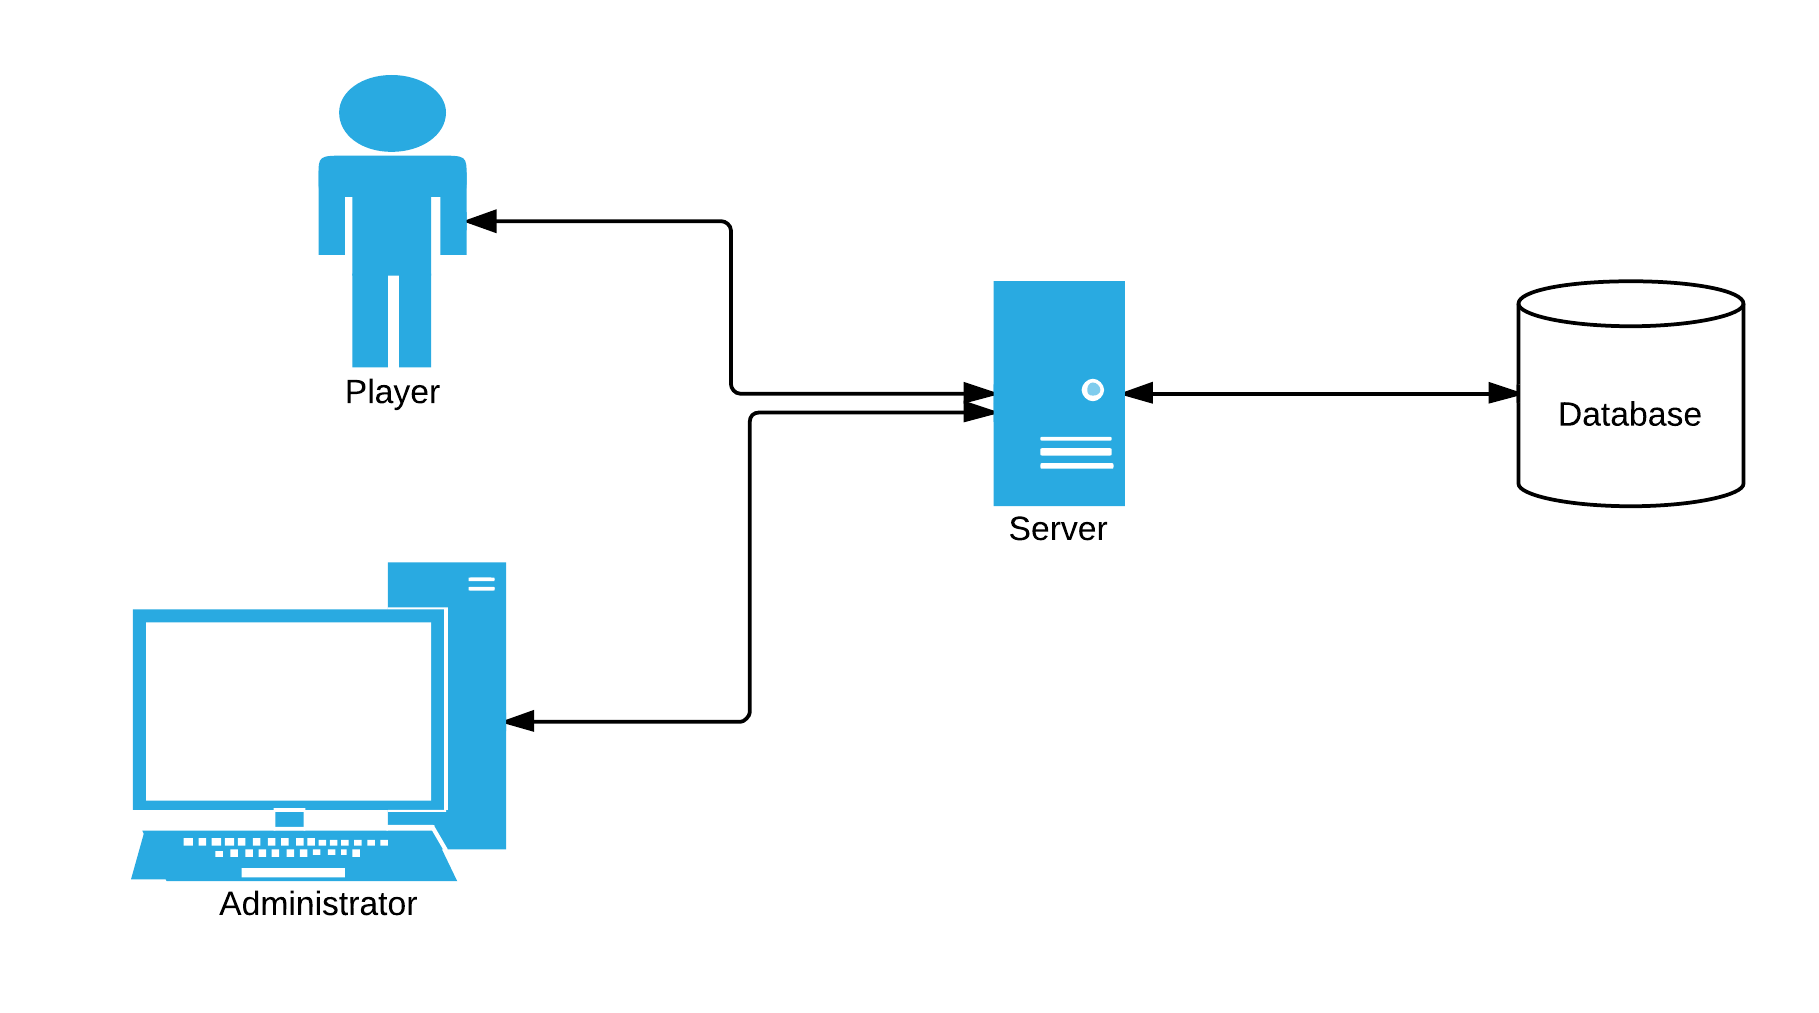
\includegraphics[width=10cm]{model.png}
  \caption{Application architecture}
  \label{Figure:fig33}
\end{figure}

\section{User Interface}
User interface is an integrated layer offering communication and logic operations between clients and machines. It is the surface of an application which can leave a good expression for users. User-friendly, comfort and easily used are its principles which could provide users convenience and efficient interaction with computers.



\subsection{Administrator}
As can be seen in \fref{Figure:fig35}, logging on to the administrator window, there should be a drop-down list to choose among showing all users, users on request and users who have been approved to participate in the game. By picking up different choices, relevant tables should be shown below the drop-down list, containing various operations the administrator can do. For example, in the user-on-request table, deletion and agreement can be executed and they should be implemented as buttons after every record. When clicking on the button, action will be activated and executed.
\begin{figure}[!htb]
  \centering
  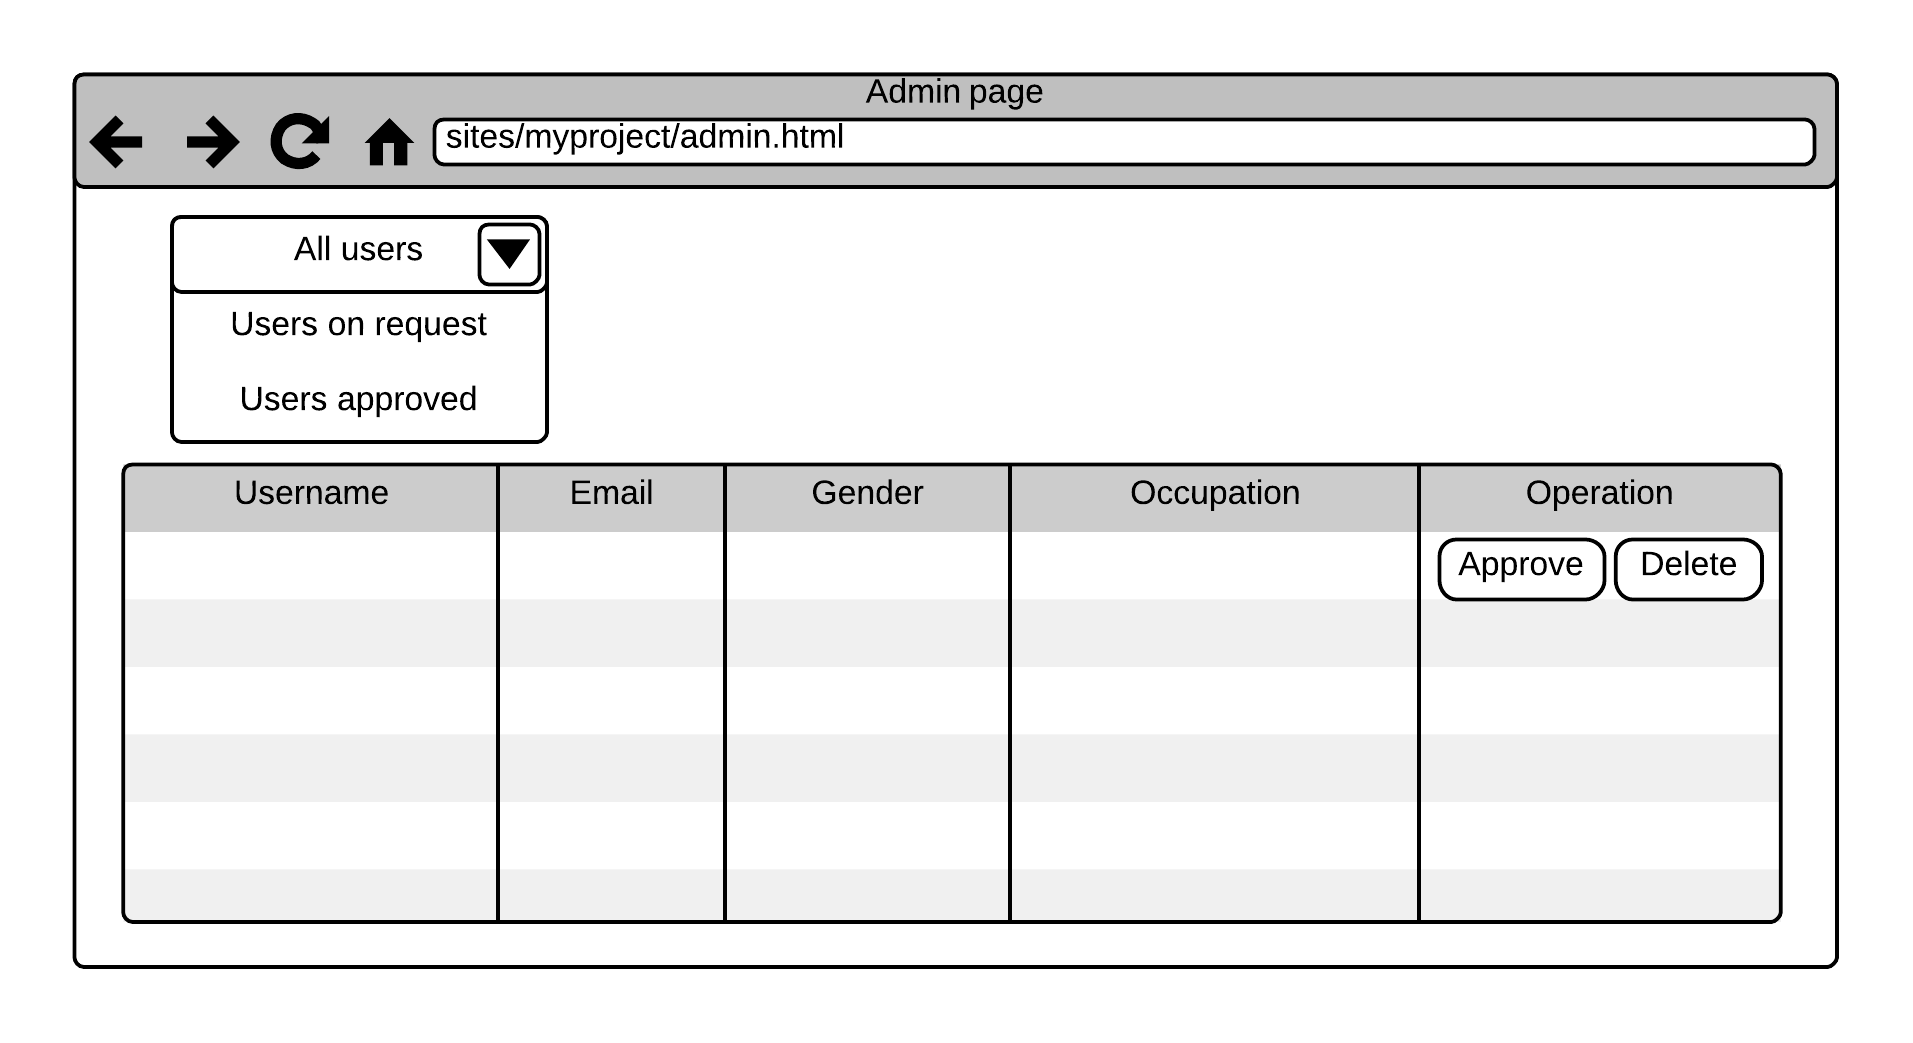
\includegraphics[width=11cm]{admin_page.png}
  \caption{Administrator page}
  \label{Figure:fig35}
\end{figure}

\subsection{Normal User}
Normal users will have two key components - \textit{instruction page and main game page}. On the instruction page, content is concise and paragraphs are separated clearly. In addition, font size should be as big as 12 point typeface which can be probably distinct enough to read. For the registering part, personal detail such as username, email and occupation should be entered in text boxes, while gender could be chosen between "Male" and "Female" and it can be achieved as a "radio" label.

Furthermore, log-on page is simple that it has two text boxes for username and password and a button to log on. When the main game page is opened, it should be roughly split into four parts, as shown in \fref{Figure:fig34}. On the left top side, it is an information module, which shows messages regarding to guidance of the game. It displays the result of last round and teaches what the player should do in the next step. Below the information module, there is an icon instruction, showing meanings of diverse icons in the map. Moreover, the prisoner's dilemma matrix will be placed in it. The main map is in the middle of the whole page, which will design as a chessboard, a 10$\times$10 table. On the chessboard, black point represents defector while white point is cooperator whose colours are contrast to each other and it could offer players clear distinction of cooperators and defectors. Furthermore, an image of  a person is on behalf the location of the player all the time. The last icon on the living area is question mark and it is the occupied location but the actual strategy is unknown which will be discovered when a player migrates to be a neighbour.All the operating buttons are on the right hand side, including cooperation, defection and other control buttons. As a whole, the core of the game is in the middle which can let users focus on the game and its left side is description while the right hand side is the operation module.

\begin{figure}[!htb]
  \centering
  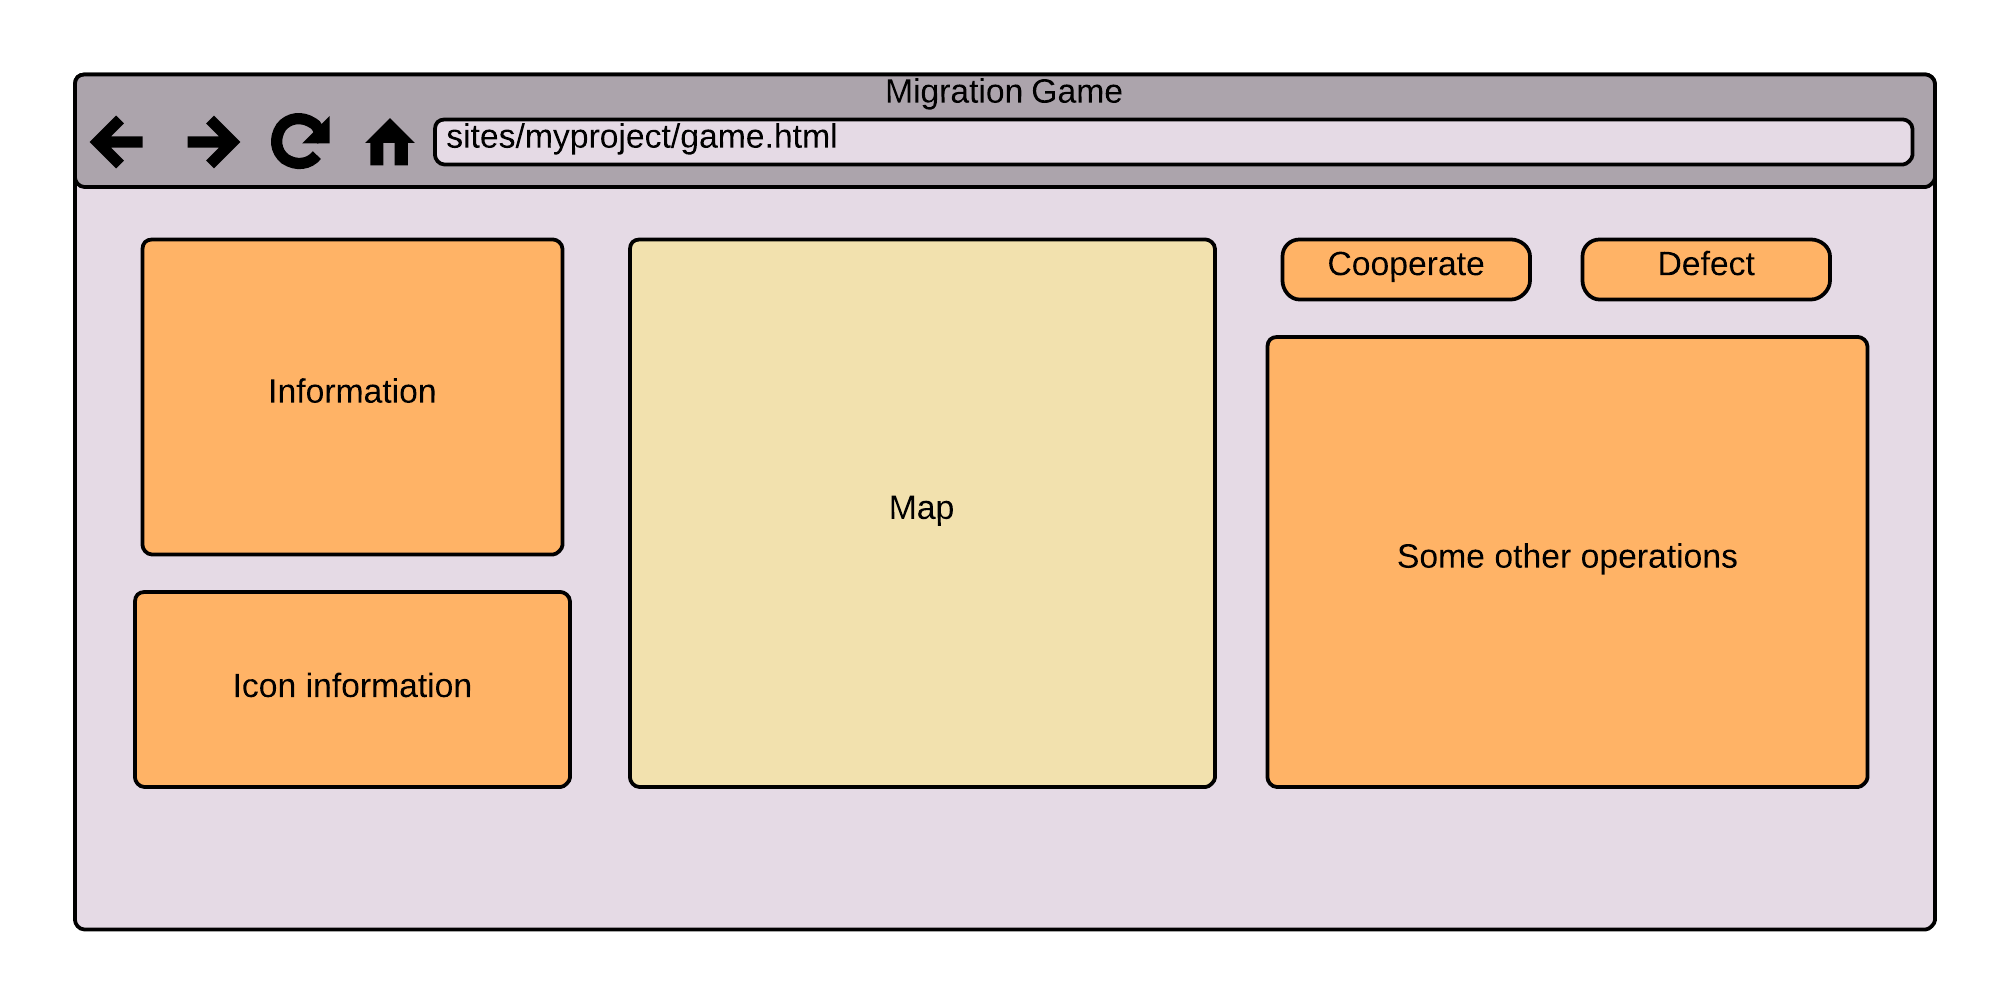
\includegraphics[width=14cm]{game_page.png}
  \caption{Game page}
  \label{Figure:fig34}
\end{figure}



\section{Business Logic Layer}

Business logic which is the core of application architecture is the connection between user interface and data access layer. A reasonable logic design is always beneficial to future maintain and extend. To be specific in the project, game procedure comes first before continuing to develop. \fref{Figure:fig32} shows the whole prcess from a user opening the webpage to storing record in the database and \fref{Figure:fig31} describes the detailed game procedure. As a whole, the procedure can be listed as follow:

\begin{figure}[!htb]
  \centering
  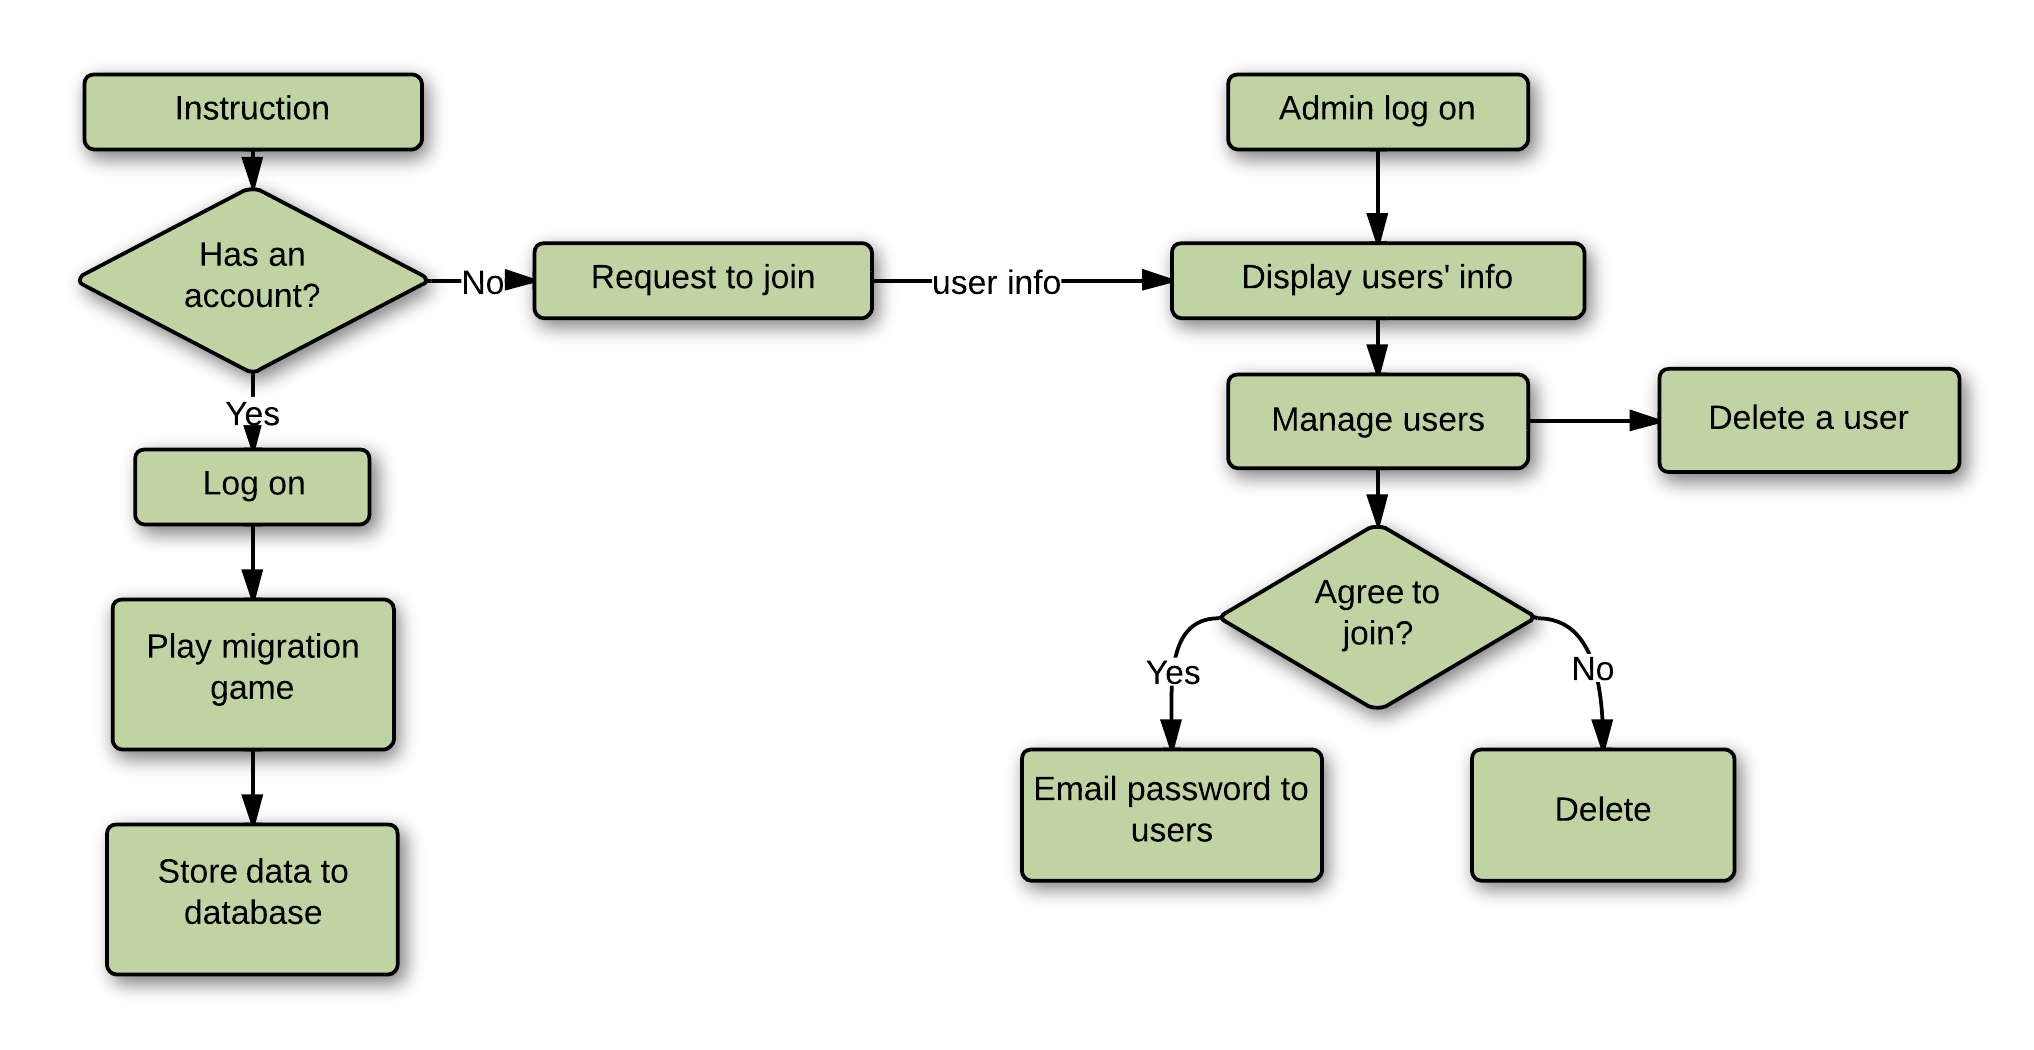
\includegraphics[width=12cm]{procedure.png}
  \caption{The whole process}
  \label{Figure:fig32}
\end{figure}

\begin{figure}[!htb]
  \centering
  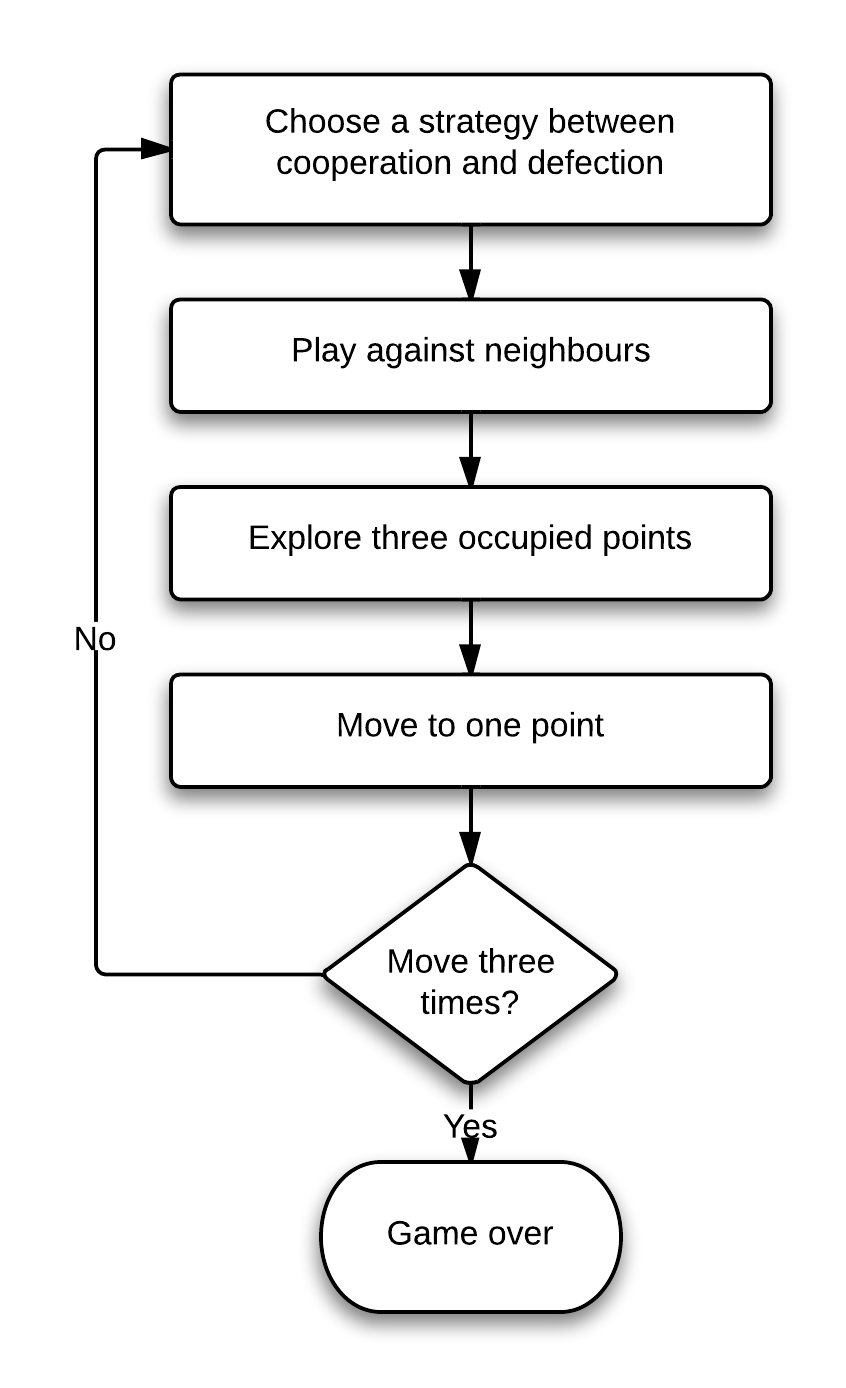
\includegraphics[width=6cm]{flow.png}
  \caption{Migration game procedure}
  \label{Figure:fig31}
\end{figure}

\begin{enumerate}
\item A user reads through the instruction of migration game and registers using his or her email address. In addition, a few personal detail should be sent as considering factors for administrators.
\item The administrator visits the managing page to monitor all the users. If a user is allowed to join the game, an email with a random password would be sent to the user which can be used to log in the game.
\item When a player enters the game, a randomised map is shown representing the living area, involving the player's initial position, occupied places whose strategies are unknown and some empty points. 
\item The player can choose the first strategy to play against his or her four neighbours and get corresponding payoff based on different combination of neighbours' strategy. The payoff matrix "abides by" prisoner's dilemma.
\item Three empty points can be explored by the player which will return corresponding bonus at this point and mark on it.
\item Move to one empty point according to exploration.
\item Users can choose strategy again and use it to play with neighbours. Then a feedback of payoff will be displayed and tell the player to continue to explore.
\item It will repeat for three times and user will get the final payoff at the end of the game.
\item All the data will be sent and stored in the database which can be visited by the administrator.
\end{enumerate}
When process is determined, how every component can be achieved should be designed next. First of all, for the instruction and register component, it is the entrance of the whole game which is able to leave a good impression for users and offer them necessary information to join the game. Detailed explanation is presented teaching people how to play the game, including what every symbol stands for. Moreover, content that the player types in should be validated before sending to the server which is definitely efficient and more secure. For example, username, email address and occupation cannot be empty and email address should be in the email format, thus the data of email can be all in same format and guarantee successful confirmation of a user's authority by email. If information is entered wrong, there will be a warning telling users to enter again. After sending the request, the user will receive a note asking to wait for the approvement. 

By clicking into the log-in page and logging on with username and password which is randomly generated, the main game will be displayed which should be split into three parts - \textit{guidance, operation and chessboard}. The guidance is responsible for showing results of the user's last action and details of what a user should do in the next step. Users play the game by hitting buttons on operation part  which will change according to the game procedure for clearly showing on which move the player is and how they can continue to play. The core of the game, chessboard, should be a 10$\times$10 table presenting the living block a person is and all manipulations directly affect and reflex on this map. In the game flow, people can choose an occupied place to explore and an empty location to move, so the map should be able to click and return some click events, such as displaying the corresponding bonus and revealing the actual strategy in a specific location. Also, each time a person move to a new place, all the neighbours should be known and payoff is automatically calculated, then how much he or she could acquire if migrating to here should be described for the user.

\section{Data Access Layer}
\begin{figure}[!htb]
	\centering
	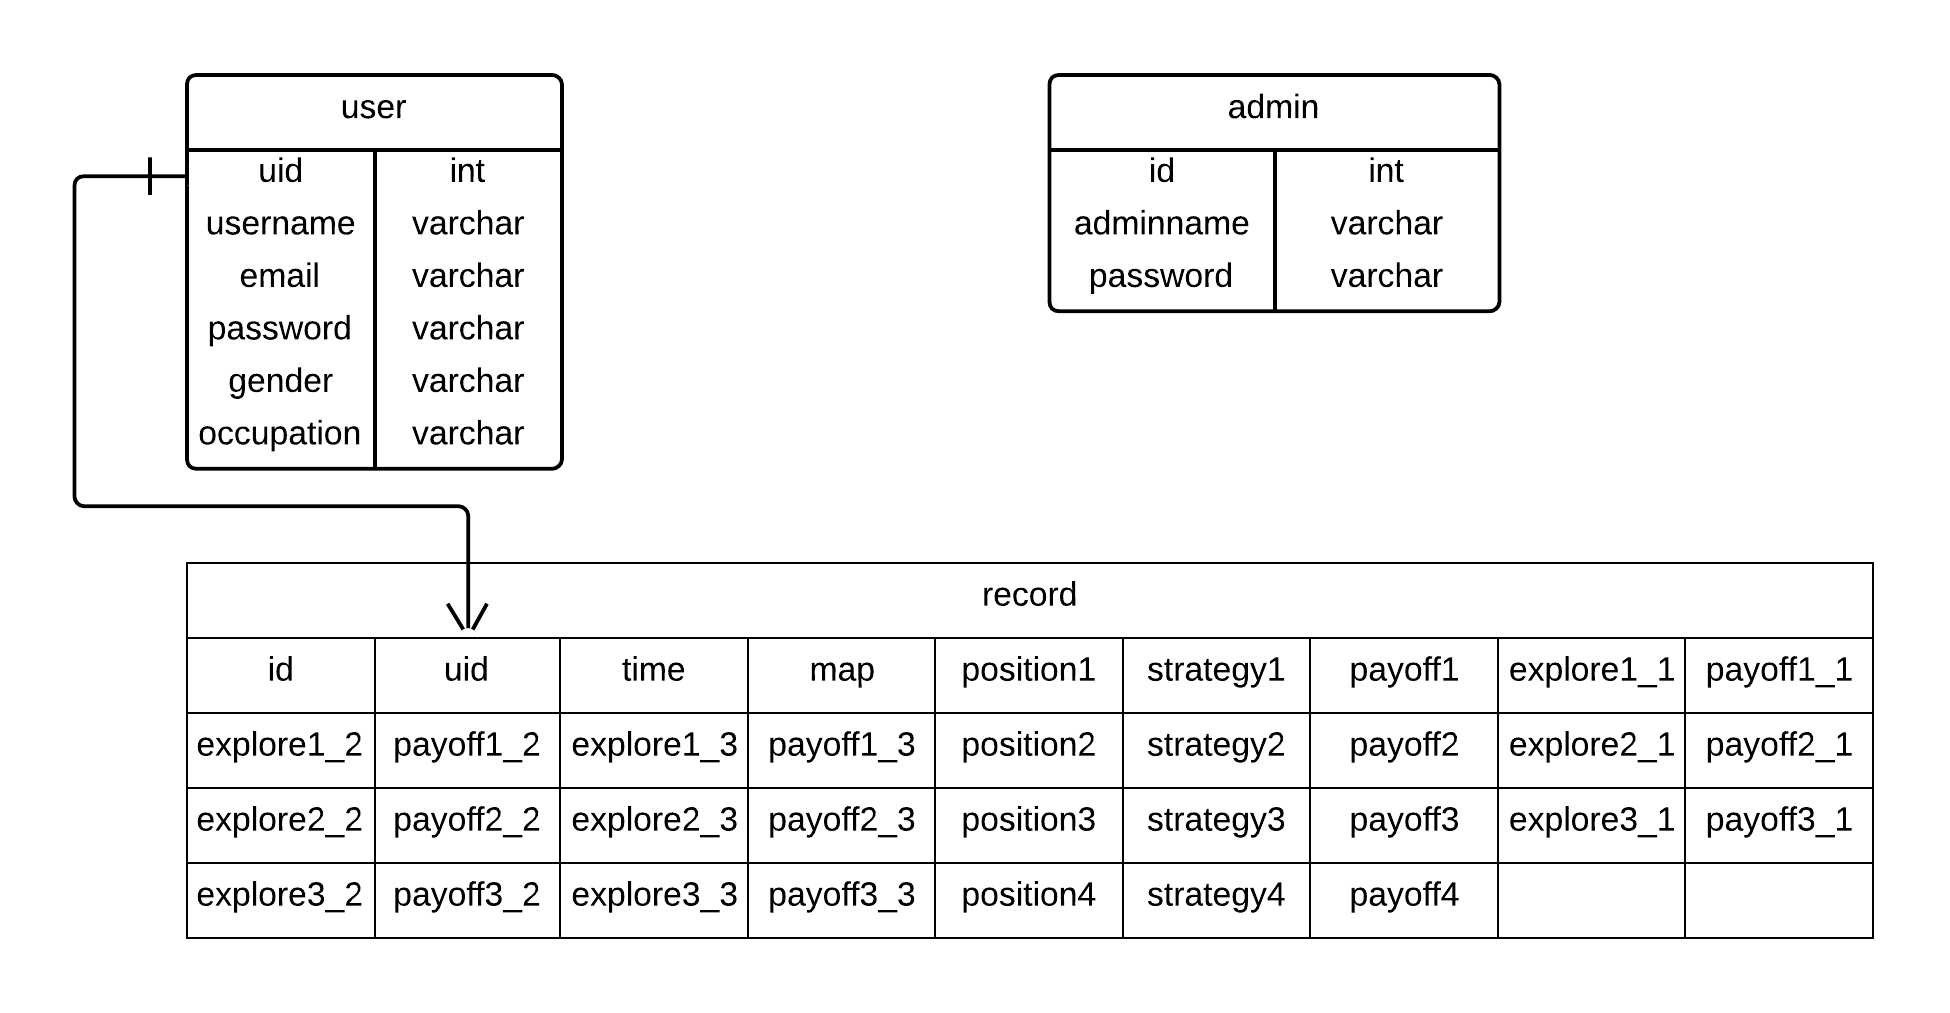
\includegraphics[width=14cm]{database.png}
	\caption{Database diagram}
	\label{Figure:figdb}
\end{figure}
The function of data access layer is to control the data flow in the database, including selecting, inserting, updating, deleting. In this project, all data is used "post" method to deliver values from html to php which is more secure. As \fref{Figure:figdb} shows, it contains three tables - \textit{user, administrator and record}.

 "Admin" has id of an administrator, name and password. When an administrator wants to log on, a select query will be executed and return the corresponding id value. If the system needs to add a new administrator, it should be directly inserted in the database which may be relatively inconvenient but more secure. 
 
The "user" table has user id, user name, email, password, gender and occupation. When a new user registers, a new record would be inserted except the password which cannot be added until the user is approved by the administrator. When he or she is agreed, a 9-digit password will be randomly generated and update the password in "md5" format which means it is encrypted and no one can read it even administrators. "State" of a user describes what status he or she is. For instance, "0" means this user has not been agreed while "1" represents the opposite meaning. In addition, user log-on action will activate a select query to test if the typed username and password exist. If the user exists, it will return the id value. Otherwise, "null" will be sent back.

The most complicated table is the "record" which stores all the data of the game. To be specific, every game has an id and who and when plays this game. Because the map is randomly initialised at the beginning of the game, it can be saved as an array. Position 1 to 4 are the player's locations every time. Similarly, strategy and payoff each round can be saved (strategy 1 to 4 and payoff 1 to 4 respectively). Additionally, coordinates of exploration and payoff at each searching point are recorded that it should be definitely necessary for the future analysis of human strategy. All these information is only inserted at the end of the game and just can be accessed by the administrator.






